\section{Evaluation}
\label{sec:evaluation}

Tighter security results in terms of loss factors are practically meaningful only if they materialize in better concrete advantage bounds when taking the underlying assumptions into account.
In our case, this amounts to the question:
How does the overall concrete security of the \SIGMA/\SIGMAI and the TLS~1.3 key exchange protocols improve based on our tighter security proofs?

\iffull
\paragraph{Parameter selection}
\else
\subsubsection*{Parameter selection\lncsdot}
\fi

In order to evaluate our and prior bounds pratically, we need to make concrete choices for each of the parameters entering the bounds.
Let us explain the choices we made in our evaluation:
\begin{description}
	\item[Runtime $t \in \{2^{40}, 2^{60}, 2^{80}\}$.]
	We parameterize the adversary's runtime between well within computational reach ($2^{40}$) and large-scale attackers ($2^{80}$).
	
	\item[Number of users $\#U = \qNewUser \in \{2^{20}, 2^{30}\}$.]
	We consider the number of users a global-scale adversary may interact with to be in the order of active public-key certificates on the Internet, reported at 130--150 million%
	\footnote{\url{https://letsencrypt.org/stats/},						%% last checked 2020-09-03: 136M active certs, 227M fully-qualified domains certified
	\url{https://trends.builtwith.com/ssl/traffic/Entire-Internet}}		%% last checked 2020-09-03: 150M detected certs
	($\approx 2^{27}$).
	
	\item[Number of sessions $\#S \approx \qSend \in \{2^{35}, 2^{45}, 2^{55}\}$.]
	Chrome%
	\fullonly{\footnote{\url{https://transparencyreport.google.com/https/}}}		%% last checked 2020-09-03: 76% -- 98%
	and Firefox%
	\fullonly{\footnote{\url{https://telemetry.mozilla.org/}}}				%% last checked 2020-09-03: 89%  (HTTP_PAGELOAD_IS_SSL)
	report that $76$--$98$\% of all web page accesses through these browsers are encrypted,
	with an active daily base of about $2$~billion ($\approx 2^{30}$) users.%
% 	Telemetry for Firefox Desktop alone reports $7.5$ million ($2^{27}$) daily pageloads through HTTPS. This number represents one day's usage for fraction of Firefox Desktop users. When we include encrypted traffic from other browsers, mobile apps, servers, and IoT devices, the number of daily sessions will be substantially higher.
	We consider adversaries may easily see $2^{35}$ sessions and a global-scale attacker may have access to $2^{55}$ sessions over an extended timespan.
	Note that the number of send queries essentially corresponds to the number of sessions.
	
	\item[Number of RO queries $\#RO = \qRO = \tfrac{t}{2^{10}}$.]
	We fix this bound at a $2^{10}$-fraction of the overall runtime accounting for all adversarial steps.
	
	\item[Diffie--Hellman groups and group order~$p$.]
	We consider all five elliptic curves standardized for \fullonly{use with }TLS~1.3 (bit-security \fullonly{level }$b$\fullelse{ and group}{, } order $p$ in parentheses):
	\texttt{secp256r1} ($b = 128$, $p \approx 2^{256}$), % source for secp256r1: https://doi.org/10.6028/NIST.FIPS.186-4 --- page 91 / Section D.1.2.3 (group order is "n")
	\texttt{secp384r1} ($b = 192$, $p \approx 2^{384}$), % source for secp284r1: https://doi.org/10.6028/NIST.FIPS.186-4 --- page 91 / Section D.1.2.4 (group order is "n")
	\texttt{secp521r1} ($b = 256$, $p \approx 2^{521}$), % source for secp521r1: https://doi.org/10.6028/NIST.FIPS.186-4 --- page 92 / Section D.1.2.5 (group order is "n")
	\texttt{x25519} ($b = 128$, $p \approx 2^{252}$), and % source for x25519: https://cr.yp.to/ecdh/curve25519-20060209.pdf --- page 8 "The order of the base point is a prime, namely 2^252 + 27742317777372353535851937790883648493."
	\texttt{x448} ($b = 224$, $p \approx 2^{446}$). % source for x448: https://eprint.iacr.org/2015/625.pdf --- page 5 "The base point ... has order q = 2^446 - ..."
	We focus on elliptic curve groups\fullonly{ only}, as they provide high efficiency and the best known algorithms for solving discrete-log and DH problems are generic,
	allowing us to apply GGM bounds for \fullelse{the involved DDH and strong DH assumptions}{DDH and strong DH}.
% 	\TODO{Fixed $p$'s for p256/p521, experiments re-run. @HD: Please double-check.}

	
	\item[Signature schemes.]
	In order to unify the underlying hardness assumptions, we consider the ECDSA/EdDSA signature schemes standardized for use with TLS~1.3, based on the five elliptic curves above,
	treating their single-user unforgeability as equally hard as the corresponding discrete logarithm\fullonly{ problem}.
	
	\item[Symmetric schemes and key/output/nonce lengths $\kl, \ol, \nl$.]% $\kl = \ol \in \{256,384\}$, $\nl = 256$.] %$\kl = \nl = \ol$.]
% 	~\lncsforcebreak
	Since our focus is mostly on evaluating ECDH parameters,
	we idealize the symmetric primitives (PRF, MAC, and hash function) in the random oracle model.
	Applying lengths standardized for TLS~1.3, we set the key and output length to $\kl = \ol = 256$~bits for $128$-bit security curves and $384$~bits for higher-security curves, corresponding to ciphersuites using SHA-256 or SHA-384.
	The nonce length is fixed to~$\nl = 256$~bits, again as in TLS~1.3.
	
% 	We consider two choices:
% 	primarily (esp.\ in Table~\ref{tbl:bounds-overview}), we consider symmetric lengths doubling the elliptic curve security level~$b$, i.e., $\kl = \nl = \ol = 2 \cdot b$.
% 	Since however four of the five cipher suites standardized for TLS~1.3 fix $256$-bit symmetric parameters,
% 	we additionally consider this variant (in Appendix~\ref{apx:evaluation:bounds-tables}).
	
	\item[Reveal and Test queries $\qRevSessionKey$, $\qRevLongTermKey$, $\qTest$.]
	Using a generic reduction to single-user signature unforgeability, the number of $\RevLongTermKey$, $\RevSessionKey$, and $\Test$ queries do not affect the bounds;
	we hence do not place any constraints on them.
\end{description}

\begin{table}[p]
	\centering
	\fontsize{4.5}{5}\selectfont % smaller than \tiny
	\renewcommand{\arraystretch}{0.01}
	\renewcommand{\tabcolsep}{0.15cm}
	\vspace{-0.5cm} %% a little higher
	\begin{tabular}{@{}lllllllllll@{}}
	\toprule
	\multicolumn{4}{c}{Adv.\ resources}		&&		& \multicolumn{2}{c}{\SIGMA}	&& \multicolumn{2}{c}{TLS~1.3} \\
	\cmidrule{1-4} \cmidrule{7-8} \cmidrule{10-11}
	$t$	& $\#U$	& $\#S$ & $\#RO$ & Curve (\fullelse{bit security~$b$, group order~$p$}{bit sec.\!~$b$,\! order~$p$})	& Target $t/2^b$	& CK\,{\cite{C:CanKra02}}~	& Us~{(Thm.~\ref{thm:SIGMAI})}	&& DFGS\,{\cite{JC:DFGS21}}~	& Us~{(Thm.~\ref{thm:tls})} \\
\midrule
$2^{40}$	&$2^{20}$	&$2^{35}$	&$2^{30}$	&\texttt{secp256r1} ($b \!=\! 128$,\! $p \!\approx\! 2^{256}$)	&$2^{-88}$	&$\approx 2^{-101}$	& $\approx 2^{-156}$	&& $\approx 2^{-104}$	& $\approx 2^{-156}$	 \\
$2^{40}$	&$2^{20}$	&$2^{45}$	&$2^{30}$	&\texttt{secp256r1} ($b \!=\! 128$,\! $p \!\approx\! 2^{256}$)	&$2^{-88}$	&$\approx 2^{-91}$	& $\approx 2^{-156}$	&& \cellcolor{red!25}$\approx 2^{-84}$	&$\approx 2^{-156}$	 \\
$2^{40}$	&$2^{20}$	&$2^{55}$	&$2^{30}$	&\texttt{secp256r1} ($b \!=\! 128$,\! $p \!\approx\! 2^{256}$)	&$2^{-88}$	&\cellcolor{red!25}$\approx 2^{-81}$	&$\approx 2^{-156}$	&& \cellcolor{red!25}$\approx 2^{-64}$	&$\approx 2^{-156}$	 \\
$2^{40}$	&$2^{30}$	&$2^{35}$	&$2^{30}$	&\texttt{secp256r1} ($b \!=\! 128$,\! $p \!\approx\! 2^{256}$)	&$2^{-88}$	&\cellcolor{red!25}$\approx 2^{-81}$	&$\approx 2^{-146}$	&& $\approx 2^{-104}$	& $\approx 2^{-146}$	 \\
$2^{40}$	&$2^{30}$	&$2^{45}$	&$2^{30}$	&\texttt{secp256r1} ($b \!=\! 128$,\! $p \!\approx\! 2^{256}$)	&$2^{-88}$	&\cellcolor{red!25}$\approx 2^{-71}$	&$\approx 2^{-146}$	&& \cellcolor{red!25}$\approx 2^{-84}$	&$\approx 2^{-146}$	 \\
$2^{40}$	&$2^{30}$	&$2^{55}$	&$2^{30}$	&\texttt{secp256r1} ($b \!=\! 128$,\! $p \!\approx\! 2^{256}$)	&$2^{-88}$	&\cellcolor{red!25}$\approx 2^{-61}$	&$\approx 2^{-146}$	&& \cellcolor{red!25}$\approx 2^{-64}$	&$\approx 2^{-146}$	 \\
\midrule
$2^{40}$	&$2^{20}$	&$2^{35}$	&$2^{30}$	&\texttt{secp384r1} ($b \!=\! 192$,\! $p \!\approx\! 2^{384}$)	&$2^{-152}$	&$\approx 2^{-229}$	& $\approx 2^{-284}$	&& $\approx 2^{-232}$	& $\approx 2^{-284}$	 \\
$2^{40}$	&$2^{20}$	&$2^{45}$	&$2^{30}$	&\texttt{secp384r1} ($b \!=\! 192$,\! $p \!\approx\! 2^{384}$)	&$2^{-152}$	&$\approx 2^{-219}$	& $\approx 2^{-284}$	&& $\approx 2^{-212}$	& $\approx 2^{-284}$	 \\
$2^{40}$	&$2^{20}$	&$2^{55}$	&$2^{30}$	&\texttt{secp384r1} ($b \!=\! 192$,\! $p \!\approx\! 2^{384}$)	&$2^{-152}$	&$\approx 2^{-209}$	& $\approx 2^{-284}$	&& $\approx 2^{-192}$	& $\approx 2^{-284}$	 \\
$2^{40}$	&$2^{30}$	&$2^{35}$	&$2^{30}$	&\texttt{secp384r1} ($b \!=\! 192$,\! $p \!\approx\! 2^{384}$)	&$2^{-152}$	&$\approx 2^{-209}$	& $\approx 2^{-274}$	&& $\approx 2^{-232}$	& $\approx 2^{-274}$	 \\
$2^{40}$	&$2^{30}$	&$2^{45}$	&$2^{30}$	&\texttt{secp384r1} ($b \!=\! 192$,\! $p \!\approx\! 2^{384}$)	&$2^{-152}$	&$\approx 2^{-199}$	& $\approx 2^{-274}$	&& $\approx 2^{-212}$	& $\approx 2^{-274}$	 \\
$2^{40}$	&$2^{30}$	&$2^{55}$	&$2^{30}$	&\texttt{secp384r1} ($b \!=\! 192$,\! $p \!\approx\! 2^{384}$)	&$2^{-152}$	&$\approx 2^{-189}$	& $\approx 2^{-274}$	&& $\approx 2^{-192}$	& $\approx 2^{-274}$	 \\
\midrule
$2^{40}$	&$2^{20}$	&$2^{35}$	&$2^{30}$	&\texttt{secp521r1} ($b \!=\! 256$,\! $p \!\approx\! 2^{521}$)	&$2^{-216}$	&$\approx 2^{-298}$	& $\approx 2^{-318}$	&& $\approx 2^{-282}$	& $\approx 2^{-317}$	 \\
$2^{40}$	&$2^{20}$	&$2^{45}$	&$2^{30}$	&\texttt{secp521r1} ($b \!=\! 256$,\! $p \!\approx\! 2^{521}$)	&$2^{-216}$	&$\approx 2^{-288}$	& $\approx 2^{-308}$	&& $\approx 2^{-262}$	& $\approx 2^{-307}$	 \\
$2^{40}$	&$2^{20}$	&$2^{55}$	&$2^{30}$	&\texttt{secp521r1} ($b \!=\! 256$,\! $p \!\approx\! 2^{521}$)	&$2^{-216}$	&$\approx 2^{-278}$	& $\approx 2^{-298}$	&& $\approx 2^{-242}$	& $\approx 2^{-297}$	 \\
$2^{40}$	&$2^{30}$	&$2^{35}$	&$2^{30}$	&\texttt{secp521r1} ($b \!=\! 256$,\! $p \!\approx\! 2^{521}$)	&$2^{-216}$	&$\approx 2^{-288}$	& $\approx 2^{-318}$	&& $\approx 2^{-282}$	& $\approx 2^{-317}$	 \\
$2^{40}$	&$2^{30}$	&$2^{45}$	&$2^{30}$	&\texttt{secp521r1} ($b \!=\! 256$,\! $p \!\approx\! 2^{521}$)	&$2^{-216}$	&$\approx 2^{-278}$	& $\approx 2^{-308}$	&& $\approx 2^{-262}$	& $\approx 2^{-307}$	 \\
$2^{40}$	&$2^{30}$	&$2^{55}$	&$2^{30}$	&\texttt{secp521r1} ($b \!=\! 256$,\! $p \!\approx\! 2^{521}$)	&$2^{-216}$	&$\approx 2^{-268}$	& $\approx 2^{-298}$	&& $\approx 2^{-242}$	& $\approx 2^{-297}$	 \\
\midrule
$2^{40}$	&$2^{20}$	&$2^{35}$	&$2^{30}$	&\texttt{x25519} ($b \!=\! 128$,\! $p \!\approx\! 2^{252}$)	&$2^{-88}$	&$\approx 2^{-97}$	& $\approx 2^{-152}$	&& $\approx 2^{-100}$	& $\approx 2^{-152}$	 \\
$2^{40}$	&$2^{20}$	&$2^{45}$	&$2^{30}$	&\texttt{x25519} ($b \!=\! 128$,\! $p \!\approx\! 2^{252}$)	&$2^{-88}$	&\cellcolor{red!25}$\approx 2^{-87}$	&$\approx 2^{-152}$	&& \cellcolor{red!25}$\approx 2^{-80}$	&$\approx 2^{-152}$	 \\
$2^{40}$	&$2^{20}$	&$2^{55}$	&$2^{30}$	&\texttt{x25519} ($b \!=\! 128$,\! $p \!\approx\! 2^{252}$)	&$2^{-88}$	&\cellcolor{red!25}$\approx 2^{-77}$	&$\approx 2^{-152}$	&& \cellcolor{red!25}$\approx 2^{-60}$	&$\approx 2^{-152}$	 \\
$2^{40}$	&$2^{30}$	&$2^{35}$	&$2^{30}$	&\texttt{x25519} ($b \!=\! 128$,\! $p \!\approx\! 2^{252}$)	&$2^{-88}$	&\cellcolor{red!25}$\approx 2^{-77}$	&$\approx 2^{-142}$	&& $\approx 2^{-100}$	& $\approx 2^{-142}$	 \\
$2^{40}$	&$2^{30}$	&$2^{45}$	&$2^{30}$	&\texttt{x25519} ($b \!=\! 128$,\! $p \!\approx\! 2^{252}$)	&$2^{-88}$	&\cellcolor{red!25}$\approx 2^{-67}$	&$\approx 2^{-142}$	&& \cellcolor{red!25}$\approx 2^{-80}$	&$\approx 2^{-142}$	 \\
$2^{40}$	&$2^{30}$	&$2^{55}$	&$2^{30}$	&\texttt{x25519} ($b \!=\! 128$,\! $p \!\approx\! 2^{252}$)	&$2^{-88}$	&\cellcolor{red!25}$\approx 2^{-57}$	&$\approx 2^{-142}$	&& \cellcolor{red!25}$\approx 2^{-60}$	&$\approx 2^{-142}$	 \\
\midrule
$2^{40}$	&$2^{20}$	&$2^{35}$	&$2^{30}$	&\texttt{x448} ($b \!=\! 224$,\! $p \!\approx\! 2^{446}$)	&$2^{-184}$	&$\approx 2^{-291}$	& $\approx 2^{-318}$	&& $\approx 2^{-282}$	& $\approx 2^{-317}$	 \\
$2^{40}$	&$2^{20}$	&$2^{45}$	&$2^{30}$	&\texttt{x448} ($b \!=\! 224$,\! $p \!\approx\! 2^{446}$)	&$2^{-184}$	&$\approx 2^{-281}$	& $\approx 2^{-308}$	&& $\approx 2^{-262}$	& $\approx 2^{-307}$	 \\
$2^{40}$	&$2^{20}$	&$2^{55}$	&$2^{30}$	&\texttt{x448} ($b \!=\! 224$,\! $p \!\approx\! 2^{446}$)	&$2^{-184}$	&$\approx 2^{-271}$	& $\approx 2^{-298}$	&& $\approx 2^{-242}$	& $\approx 2^{-297}$	 \\
$2^{40}$	&$2^{30}$	&$2^{35}$	&$2^{30}$	&\texttt{x448} ($b \!=\! 224$,\! $p \!\approx\! 2^{446}$)	&$2^{-184}$	&$\approx 2^{-271}$	& $\approx 2^{-318}$	&& $\approx 2^{-282}$	& $\approx 2^{-317}$	 \\
$2^{40}$	&$2^{30}$	&$2^{45}$	&$2^{30}$	&\texttt{x448} ($b \!=\! 224$,\! $p \!\approx\! 2^{446}$)	&$2^{-184}$	&$\approx 2^{-261}$	& $\approx 2^{-308}$	&& $\approx 2^{-262}$	& $\approx 2^{-307}$	 \\
$2^{40}$	&$2^{30}$	&$2^{55}$	&$2^{30}$	&\texttt{x448} ($b \!=\! 224$,\! $p \!\approx\! 2^{446}$)	&$2^{-184}$	&$\approx 2^{-251}$	& $\approx 2^{-298}$	&& $\approx 2^{-242}$	& $\approx 2^{-297}$	 \\
\midrule
\midrule
$2^{60}$	&$2^{20}$	&$2^{35}$	&$2^{50}$	&\texttt{secp256r1} ($b \!=\! 128$,\! $p \!\approx\! 2^{256}$)	&$2^{-68}$	&\cellcolor{red!25}$\approx 2^{-61}$	&$\approx 2^{-116}$	&& \cellcolor{red!25}$\approx 2^{-64}$	&$\approx 2^{-116}$	 \\
$2^{60}$	&$2^{20}$	&$2^{45}$	&$2^{50}$	&\texttt{secp256r1} ($b \!=\! 128$,\! $p \!\approx\! 2^{256}$)	&$2^{-68}$	&\cellcolor{red!25}$\approx 2^{-51}$	&$\approx 2^{-116}$	&& \cellcolor{red!25}$\approx 2^{-44}$	&$\approx 2^{-116}$	 \\
$2^{60}$	&$2^{20}$	&$2^{55}$	&$2^{50}$	&\texttt{secp256r1} ($b \!=\! 128$,\! $p \!\approx\! 2^{256}$)	&$2^{-68}$	&\cellcolor{red!25}$\approx 2^{-41}$	&$\approx 2^{-116}$	&& \cellcolor{red!25}$\approx 2^{-24}$	&$\approx 2^{-116}$	 \\
$2^{60}$	&$2^{30}$	&$2^{35}$	&$2^{50}$	&\texttt{secp256r1} ($b \!=\! 128$,\! $p \!\approx\! 2^{256}$)	&$2^{-68}$	&\cellcolor{red!25}$\approx 2^{-41}$	&$\approx 2^{-106}$	&& \cellcolor{red!25}$\approx 2^{-64}$	&$\approx 2^{-106}$	 \\
$2^{60}$	&$2^{30}$	&$2^{45}$	&$2^{50}$	&\texttt{secp256r1} ($b \!=\! 128$,\! $p \!\approx\! 2^{256}$)	&$2^{-68}$	&\cellcolor{red!25}$\approx 2^{-31}$	&$\approx 2^{-106}$	&& \cellcolor{red!25}$\approx 2^{-44}$	&$\approx 2^{-106}$	 \\
$2^{60}$	&$2^{30}$	&$2^{55}$	&$2^{50}$	&\texttt{secp256r1} ($b \!=\! 128$,\! $p \!\approx\! 2^{256}$)	&$2^{-68}$	&\cellcolor{red!25}$\approx 2^{-21}$	&$\approx 2^{-106}$	&& \cellcolor{red!25}$\approx 2^{-24}$	&$\approx 2^{-106}$	 \\
\midrule
$2^{60}$	&$2^{20}$	&$2^{35}$	&$2^{50}$	&\texttt{secp384r1} ($b \!=\! 192$,\! $p \!\approx\! 2^{384}$)	&$2^{-132}$	&$\approx 2^{-189}$	& $\approx 2^{-244}$	&& $\approx 2^{-192}$	& $\approx 2^{-244}$	 \\
$2^{60}$	&$2^{20}$	&$2^{45}$	&$2^{50}$	&\texttt{secp384r1} ($b \!=\! 192$,\! $p \!\approx\! 2^{384}$)	&$2^{-132}$	&$\approx 2^{-179}$	& $\approx 2^{-244}$	&& $\approx 2^{-172}$	& $\approx 2^{-244}$	 \\
$2^{60}$	&$2^{20}$	&$2^{55}$	&$2^{50}$	&\texttt{secp384r1} ($b \!=\! 192$,\! $p \!\approx\! 2^{384}$)	&$2^{-132}$	&$\approx 2^{-169}$	& $\approx 2^{-244}$	&& $\approx 2^{-152}$	& $\approx 2^{-244}$	 \\
$2^{60}$	&$2^{30}$	&$2^{35}$	&$2^{50}$	&\texttt{secp384r1} ($b \!=\! 192$,\! $p \!\approx\! 2^{384}$)	&$2^{-132}$	&$\approx 2^{-169}$	& $\approx 2^{-234}$	&& $\approx 2^{-192}$	& $\approx 2^{-234}$	 \\
$2^{60}$	&$2^{30}$	&$2^{45}$	&$2^{50}$	&\texttt{secp384r1} ($b \!=\! 192$,\! $p \!\approx\! 2^{384}$)	&$2^{-132}$	&$\approx 2^{-159}$	& $\approx 2^{-234}$	&& $\approx 2^{-172}$	& $\approx 2^{-234}$	 \\
$2^{60}$	&$2^{30}$	&$2^{55}$	&$2^{50}$	&\texttt{secp384r1} ($b \!=\! 192$,\! $p \!\approx\! 2^{384}$)	&$2^{-132}$	&$\approx 2^{-149}$	& $\approx 2^{-234}$	&& $\approx 2^{-152}$	& $\approx 2^{-234}$	 \\
\midrule
$2^{60}$	&$2^{20}$	&$2^{35}$	&$2^{50}$	&\texttt{secp521r1} ($b \!=\! 256$,\! $p \!\approx\! 2^{521}$)	&$2^{-196}$	&$\approx 2^{-278}$	& $\approx 2^{-298}$	&& $\approx 2^{-250}$	& $\approx 2^{-285}$	 \\
$2^{60}$	&$2^{20}$	&$2^{45}$	&$2^{50}$	&\texttt{secp521r1} ($b \!=\! 256$,\! $p \!\approx\! 2^{521}$)	&$2^{-196}$	&$\approx 2^{-268}$	& $\approx 2^{-288}$	&& $\approx 2^{-240}$	& $\approx 2^{-285}$	 \\
$2^{60}$	&$2^{20}$	&$2^{55}$	&$2^{50}$	&\texttt{secp521r1} ($b \!=\! 256$,\! $p \!\approx\! 2^{521}$)	&$2^{-196}$	&$\approx 2^{-258}$	& $\approx 2^{-278}$	&& $\approx 2^{-222}$	& $\approx 2^{-277}$	 \\
$2^{60}$	&$2^{30}$	&$2^{35}$	&$2^{50}$	&\texttt{secp521r1} ($b \!=\! 256$,\! $p \!\approx\! 2^{521}$)	&$2^{-196}$	&$\approx 2^{-268}$	& $\approx 2^{-298}$	&& $\approx 2^{-250}$	& $\approx 2^{-285}$	 \\
$2^{60}$	&$2^{30}$	&$2^{45}$	&$2^{50}$	&\texttt{secp521r1} ($b \!=\! 256$,\! $p \!\approx\! 2^{521}$)	&$2^{-196}$	&$\approx 2^{-258}$	& $\approx 2^{-288}$	&& $\approx 2^{-240}$	& $\approx 2^{-285}$	 \\
$2^{60}$	&$2^{30}$	&$2^{55}$	&$2^{50}$	&\texttt{secp521r1} ($b \!=\! 256$,\! $p \!\approx\! 2^{521}$)	&$2^{-196}$	&$\approx 2^{-248}$	& $\approx 2^{-278}$	&& $\approx 2^{-222}$	& $\approx 2^{-277}$	 \\
\midrule
$2^{60}$	&$2^{20}$	&$2^{35}$	&$2^{50}$	&\texttt{x25519} ($b \!=\! 128$,\! $p \!\approx\! 2^{252}$)	&$2^{-68}$	&\cellcolor{red!25}$\approx 2^{-57}$	&$\approx 2^{-112}$	&& \cellcolor{red!25}$\approx 2^{-60}$	&$\approx 2^{-112}$	 \\
$2^{60}$	&$2^{20}$	&$2^{45}$	&$2^{50}$	&\texttt{x25519} ($b \!=\! 128$,\! $p \!\approx\! 2^{252}$)	&$2^{-68}$	&\cellcolor{red!25}$\approx 2^{-47}$	&$\approx 2^{-112}$	&& \cellcolor{red!25}$\approx 2^{-40}$	&$\approx 2^{-112}$	 \\
$2^{60}$	&$2^{20}$	&$2^{55}$	&$2^{50}$	&\texttt{x25519} ($b \!=\! 128$,\! $p \!\approx\! 2^{252}$)	&$2^{-68}$	&\cellcolor{red!25}$\approx 2^{-37}$	&$\approx 2^{-112}$	&& \cellcolor{red!25}$\approx 2^{-20}$	&$\approx 2^{-112}$	 \\
$2^{60}$	&$2^{30}$	&$2^{35}$	&$2^{50}$	&\texttt{x25519} ($b \!=\! 128$,\! $p \!\approx\! 2^{252}$)	&$2^{-68}$	&\cellcolor{red!25}$\approx 2^{-37}$	&$\approx 2^{-102}$	&& \cellcolor{red!25}$\approx 2^{-60}$	&$\approx 2^{-102}$	 \\
$2^{60}$	&$2^{30}$	&$2^{45}$	&$2^{50}$	&\texttt{x25519} ($b \!=\! 128$,\! $p \!\approx\! 2^{252}$)	&$2^{-68}$	&\cellcolor{red!25}$\approx 2^{-27}$	&$\approx 2^{-102}$	&& \cellcolor{red!25}$\approx 2^{-40}$	&$\approx 2^{-102}$	 \\
$2^{60}$	&$2^{30}$	&$2^{55}$	&$2^{50}$	&\texttt{x25519} ($b \!=\! 128$,\! $p \!\approx\! 2^{252}$)	&$2^{-68}$	&\cellcolor{red!25}$\approx 2^{-17}$	&$\approx 2^{-102}$	&& \cellcolor{red!25}$\approx 2^{-20}$	&$\approx 2^{-102}$	 \\
\midrule
$2^{60}$	&$2^{20}$	&$2^{35}$	&$2^{50}$	&\texttt{x448} ($b \!=\! 224$,\! $p \!\approx\! 2^{446}$)	&$2^{-164}$	&$\approx 2^{-251}$	& $\approx 2^{-298}$	&& $\approx 2^{-250}$	& $\approx 2^{-285}$	 \\
$2^{60}$	&$2^{20}$	&$2^{45}$	&$2^{50}$	&\texttt{x448} ($b \!=\! 224$,\! $p \!\approx\! 2^{446}$)	&$2^{-164}$	&$\approx 2^{-241}$	& $\approx 2^{-288}$	&& $\approx 2^{-234}$	& $\approx 2^{-285}$	 \\
$2^{60}$	&$2^{20}$	&$2^{55}$	&$2^{50}$	&\texttt{x448} ($b \!=\! 224$,\! $p \!\approx\! 2^{446}$)	&$2^{-164}$	&$\approx 2^{-231}$	& $\approx 2^{-278}$	&& $\approx 2^{-214}$	& $\approx 2^{-277}$	 \\
$2^{60}$	&$2^{30}$	&$2^{35}$	&$2^{50}$	&\texttt{x448} ($b \!=\! 224$,\! $p \!\approx\! 2^{446}$)	&$2^{-164}$	&$\approx 2^{-231}$	& $\approx 2^{-296}$	&& $\approx 2^{-250}$	& $\approx 2^{-285}$	 \\
$2^{60}$	&$2^{30}$	&$2^{45}$	&$2^{50}$	&\texttt{x448} ($b \!=\! 224$,\! $p \!\approx\! 2^{446}$)	&$2^{-164}$	&$\approx 2^{-221}$	& $\approx 2^{-288}$	&& $\approx 2^{-234}$	& $\approx 2^{-285}$	 \\
$2^{60}$	&$2^{30}$	&$2^{55}$	&$2^{50}$	&\texttt{x448} ($b \!=\! 224$,\! $p \!\approx\! 2^{446}$)	&$2^{-164}$	&$\approx 2^{-211}$	& $\approx 2^{-278}$	&& $\approx 2^{-214}$	& $\approx 2^{-277}$	 \\
\midrule
\midrule
$2^{80}$	&$2^{20}$	&$2^{35}$	&$2^{70}$	&\texttt{secp256r1} ($b \!=\! 128$,\! $p \!\approx\! 2^{256}$)	&$2^{-48}$	&\cellcolor{red!25}$\approx 2^{-21}$	&$\approx 2^{-76}$	&& \cellcolor{red!25}$\approx 2^{-24}$	&$\approx 2^{-76}$	 \\
$2^{80}$	&$2^{20}$	&$2^{45}$	&$2^{70}$	&\texttt{secp256r1} ($b \!=\! 128$,\! $p \!\approx\! 2^{256}$)	&$2^{-48}$	&\cellcolor{red!25}$\approx 2^{-11}$	&$\approx 2^{-76}$	&& \cellcolor{red!25}$\approx 2^{-4}$	&$\approx 2^{-76}$	 \\
$2^{80}$	&$2^{20}$	&$2^{55}$	&$2^{70}$	&\texttt{secp256r1} ($b \!=\! 128$,\! $p \!\approx\! 2^{256}$)	&$2^{-48}$	&\cellcolor{red!25}$\approx 2^{-1}$	&$\approx 2^{-76}$	&& \cellcolor{red!25}1			&$\approx 2^{-76}$	 \\
$2^{80}$	&$2^{30}$	&$2^{35}$	&$2^{70}$	&\texttt{secp256r1} ($b \!=\! 128$,\! $p \!\approx\! 2^{256}$)	&$2^{-48}$	&\cellcolor{red!25}$\approx 2^{-1}$	&$\approx 2^{-66}$	&& \cellcolor{red!25}$\approx 2^{-24}$	&$\approx 2^{-66}$	 \\
$2^{80}$	&$2^{30}$	&$2^{45}$	&$2^{70}$	&\texttt{secp256r1} ($b \!=\! 128$,\! $p \!\approx\! 2^{256}$)	&$2^{-48}$	&\cellcolor{red!25}1			&$\approx 2^{-66}$	&& \cellcolor{red!25}$\approx 2^{-4}$	&$\approx 2^{-66}$	 \\
$2^{80}$	&$2^{30}$	&$2^{55}$	&$2^{70}$	&\texttt{secp256r1} ($b \!=\! 128$,\! $p \!\approx\! 2^{256}$)	&$2^{-48}$	&\cellcolor{red!25}1			&$\approx 2^{-66}$	&& \cellcolor{red!25}1			&$\approx 2^{-66}$	 \\
\midrule
$2^{80}$	&$2^{20}$	&$2^{35}$	&$2^{70}$	&\texttt{secp384r1} ($b \!=\! 192$,\! $p \!\approx\! 2^{384}$)	&$2^{-112}$	&$\approx 2^{-149}$	& $\approx 2^{-204}$	&& $\approx 2^{-152}$	& $\approx 2^{-204}$	 \\
$2^{80}$	&$2^{20}$	&$2^{45}$	&$2^{70}$	&\texttt{secp384r1} ($b \!=\! 192$,\! $p \!\approx\! 2^{384}$)	&$2^{-112}$	&$\approx 2^{-139}$	& $\approx 2^{-204}$	&& $\approx 2^{-132}$	& $\approx 2^{-204}$	 \\
$2^{80}$	&$2^{20}$	&$2^{55}$	&$2^{70}$	&\texttt{secp384r1} ($b \!=\! 192$,\! $p \!\approx\! 2^{384}$)	&$2^{-112}$	&$\approx 2^{-129}$	& $\approx 2^{-204}$	&& \cellcolor{orange!25}$\approx 2^{-112}$	&$\approx 2^{-204}$	 \\
$2^{80}$	&$2^{30}$	&$2^{35}$	&$2^{70}$	&\texttt{secp384r1} ($b \!=\! 192$,\! $p \!\approx\! 2^{384}$)	&$2^{-112}$	&$\approx 2^{-129}$	& $\approx 2^{-194}$	&& $\approx 2^{-152}$	& $\approx 2^{-194}$	 \\
$2^{80}$	&$2^{30}$	&$2^{45}$	&$2^{70}$	&\texttt{secp384r1} ($b \!=\! 192$,\! $p \!\approx\! 2^{384}$)	&$2^{-112}$	&$\approx 2^{-119}$	& $\approx 2^{-194}$	&& $\approx 2^{-132}$	& $\approx 2^{-194}$	 \\
$2^{80}$	&$2^{30}$	&$2^{55}$	&$2^{70}$	&\texttt{secp384r1} ($b \!=\! 192$,\! $p \!\approx\! 2^{384}$)	&$2^{-112}$	&\cellcolor{red!25}$\approx 2^{-109}$	&$\approx 2^{-194}$	&& \cellcolor{orange!25}$\approx 2^{-112}$	&$\approx 2^{-194}$	 \\
\midrule
$2^{80}$	&$2^{20}$	&$2^{35}$	&$2^{70}$	&\texttt{secp521r1} ($b \!=\! 256$,\! $p \!\approx\! 2^{521}$)	&$2^{-176}$	&$\approx 2^{-258}$	& $\approx 2^{-278}$	&& $\approx 2^{-210}$	& $\approx 2^{-245}$	 \\
$2^{80}$	&$2^{20}$	&$2^{45}$	&$2^{70}$	&\texttt{secp521r1} ($b \!=\! 256$,\! $p \!\approx\! 2^{521}$)	&$2^{-176}$	&$\approx 2^{-248}$	& $\approx 2^{-268}$	&& $\approx 2^{-200}$	& $\approx 2^{-245}$	 \\
$2^{80}$	&$2^{20}$	&$2^{55}$	&$2^{70}$	&\texttt{secp521r1} ($b \!=\! 256$,\! $p \!\approx\! 2^{521}$)	&$2^{-176}$	&$\approx 2^{-238}$	& $\approx 2^{-258}$	&& $\approx 2^{-190}$	& $\approx 2^{-245}$	 \\
$2^{80}$	&$2^{30}$	&$2^{35}$	&$2^{70}$	&\texttt{secp521r1} ($b \!=\! 256$,\! $p \!\approx\! 2^{521}$)	&$2^{-176}$	&$\approx 2^{-248}$	& $\approx 2^{-278}$	&& $\approx 2^{-210}$	& $\approx 2^{-245}$	 \\
$2^{80}$	&$2^{30}$	&$2^{45}$	&$2^{70}$	&\texttt{secp521r1} ($b \!=\! 256$,\! $p \!\approx\! 2^{521}$)	&$2^{-176}$	&$\approx 2^{-238}$	& $\approx 2^{-268}$	&& $\approx 2^{-200}$	& $\approx 2^{-245}$	 \\
$2^{80}$	&$2^{30}$	&$2^{55}$	&$2^{70}$	&\texttt{secp521r1} ($b \!=\! 256$,\! $p \!\approx\! 2^{521}$)	&$2^{-176}$	&$\approx 2^{-228}$	& $\approx 2^{-258}$	&& $\approx 2^{-190}$	& $\approx 2^{-245}$	 \\
\midrule
$2^{80}$	&$2^{20}$	&$2^{35}$	&$2^{70}$	&\texttt{x25519} ($b \!=\! 128$,\! $p \!\approx\! 2^{252}$)	&$2^{-48}$	&\cellcolor{red!25}$\approx 2^{-17}$	&$\approx 2^{-72}$	&& \cellcolor{red!25}$\approx 2^{-20}$	&$\approx 2^{-72}$	 \\
$2^{80}$	&$2^{20}$	&$2^{45}$	&$2^{70}$	&\texttt{x25519} ($b \!=\! 128$,\! $p \!\approx\! 2^{252}$)	&$2^{-48}$	&\cellcolor{red!25}$\approx 2^{-7}$	&$\approx 2^{-72}$	&& \cellcolor{red!25}1			&$\approx 2^{-72}$	 \\
$2^{80}$	&$2^{20}$	&$2^{55}$	&$2^{70}$	&\texttt{x25519} ($b \!=\! 128$,\! $p \!\approx\! 2^{252}$)	&$2^{-48}$	&\cellcolor{red!25}1			&$\approx 2^{-72}$	&& \cellcolor{red!25}1			&$\approx 2^{-72}$	 \\
$2^{80}$	&$2^{30}$	&$2^{35}$	&$2^{70}$	&\texttt{x25519} ($b \!=\! 128$,\! $p \!\approx\! 2^{252}$)	&$2^{-48}$	&\cellcolor{red!25}1			&$\approx 2^{-62}$	&& \cellcolor{red!25}$\approx 2^{-20}$	&$\approx 2^{-62}$	 \\
$2^{80}$	&$2^{30}$	&$2^{45}$	&$2^{70}$	&\texttt{x25519} ($b \!=\! 128$,\! $p \!\approx\! 2^{252}$)	&$2^{-48}$	&\cellcolor{red!25}1			&$\approx 2^{-62}$	&& \cellcolor{red!25}1			&$\approx 2^{-62}$	 \\
$2^{80}$	&$2^{30}$	&$2^{55}$	&$2^{70}$	&\texttt{x25519} ($b \!=\! 128$,\! $p \!\approx\! 2^{252}$)	&$2^{-48}$	&\cellcolor{red!25}1			&$\approx 2^{-62}$	&& \cellcolor{red!25}1			&$\approx 2^{-62}$	 \\
\midrule
$2^{80}$	&$2^{20}$	&$2^{35}$	&$2^{70}$	&\texttt{x448} ($b \!=\! 224$,\! $p \!\approx\! 2^{446}$)	&$2^{-144}$	&$\approx 2^{-211}$	& $\approx 2^{-266}$	&& $\approx 2^{-210}$	& $\approx 2^{-245}$	 \\
$2^{80}$	&$2^{20}$	&$2^{45}$	&$2^{70}$	&\texttt{x448} ($b \!=\! 224$,\! $p \!\approx\! 2^{446}$)	&$2^{-144}$	&$\approx 2^{-201}$	& $\approx 2^{-266}$	&& $\approx 2^{-194}$	& $\approx 2^{-245}$	 \\
$2^{80}$	&$2^{20}$	&$2^{55}$	&$2^{70}$	&\texttt{x448} ($b \!=\! 224$,\! $p \!\approx\! 2^{446}$)	&$2^{-144}$	&$\approx 2^{-191}$	& $\approx 2^{-258}$	&& $\approx 2^{-174}$	& $\approx 2^{-245}$	 \\
$2^{80}$	&$2^{30}$	&$2^{35}$	&$2^{70}$	&\texttt{x448} ($b \!=\! 224$,\! $p \!\approx\! 2^{446}$)	&$2^{-144}$	&$\approx 2^{-191}$	& $\approx 2^{-256}$	&& $\approx 2^{-210}$	& $\approx 2^{-245}$	 \\
$2^{80}$	&$2^{30}$	&$2^{45}$	&$2^{70}$	&\texttt{x448} ($b \!=\! 224$,\! $p \!\approx\! 2^{446}$)	&$2^{-144}$	&$\approx 2^{-181}$	& $\approx 2^{-256}$	&& $\approx 2^{-194}$	& $\approx 2^{-245}$	 \\
$2^{80}$	&$2^{30}$	&$2^{55}$	&$2^{70}$	&\texttt{x448} ($b \!=\! 224$,\! $p \!\approx\! 2^{446}$)	&$2^{-144}$	&$\approx 2^{-171}$	& $\approx 2^{-256}$	&& $\approx 2^{-174}$	& $\approx 2^{-245}$	 \\
\bottomrule
	\end{tabular}
	
	\medskip
	
	\caption{%
		\fullelse{%
		Advantages of a key exchange adversary with given resources $t$ (running time), $\#U$ (number of users), $\#S$ (number of sessions), and $\#RO$ (number of random oracle queries),
		in breaking the security of the \SIGMA and TLS~1.3 protocols
		when instantiated with the given curves (bit security~$b$ and group order~$p$ in parentheses),
		based on the prior bounds by Canetti-Krawczyk~\cite{C:CanKra02} resp.\ Dowling et al.~\cite{JC:DFGS21}, and the bounds we establish (Theorem~\ref{thm:SIGMAI} and~\ref{thm:tls}).
		Target indicates the maximal advantage~$t/2^b$ tolerable when aiming for the respective curve's security level~$b$;
		entries in red-shaded cells miss that target.
		See Section~\ref{sec:evaluation} for further details.
		}{%
		Advantages of a key exchange adversary with given resources in breaking the security of the \SIGMA and TLS~1.3 protocols.
		See Section~\ref{sec:evaluation} for further details.
		}
	}
	\label{tbl:bounds-full:symmetric-256-384}
\end{table}



\iffull
\paragraph{Fully-quantitative CK/DFGS bounds for \SIGMA/TLS~1.3}
\else
\subsubsection*{Fully-quantitative CK/DFGS bounds for \SIGMA/TLS~1.3\lncsdot}
\fi

For our evaluation, we need to reconstruct fully-quantitative security bounds from the more abstract prior security proofs for \SIGMA by Canetti-Krawczyk~\cite{C:CanKra02} and for TLS~1.3 by Dowling et al.~\cite{JC:DFGS21}.
We report them in Appendix~\ref{apx:evaluation} for reference.
In terms of their reduction to underlying DH problems,
the CK \SIGMA bound reduces to the DDH problem with a loss of $\#U \cdot \#S$,
whereas the DFGS TLS~1.3 bound reduces to the strong DH problem with a loss of $(\#S)^2$.

\begin{figure}[t]
		\label{fig:required-groupsize}
	%%%
	%%% Elliptic curve group order required to achieve 128-bit resp. 192-bit AKE security
	%%% Computed via bounds.py, function p_estimates
	%%%
	
	%
	% General formulas are dominated by (adv = t / seclevel):
	%  * CK:	qn*(qn+1)*qs * t²/adv [sig2]
	%  * Our SIGMA:	qn * t²/adv [sig]
	%  * DFGS sm: 	qs*qn * t²/adv [sig]		for qs <= 2^18
	%		qs² * 4*t'²/adv [PRF-ODH]	for (128-bit AND 2^18 <= qs <= 2^68)  OR  (192-bit AND qs >= 2^18)
	%		-- unsatisfiable --		for (128-bit AND qs >= 2^68)  // due to PRF term
	%  * DFGS lg: 	qs*qn * t²/adv [sig]		for qs <= 2^25
	%		qs² * t'²/adv [PRF-ODH]		for (128-bit AND 2^28 <= qs <= 2^68)  OR  (192-bit AND qs >= 2^28)
	%		-- unsatisfiable --		for (128-bit AND qs >= 2^68)  (due to PRF term)
	%  * Our TLS:	qn * t²/adv [sig]
	%
	%  (t' = prfodh/stDH reduction time: t' =~ t+2000*qRO)
	%
	
	\begin{minipage}{\textwidth}
		
		%
		% 128 bit security
		%
		
		\hspace{2cm}
		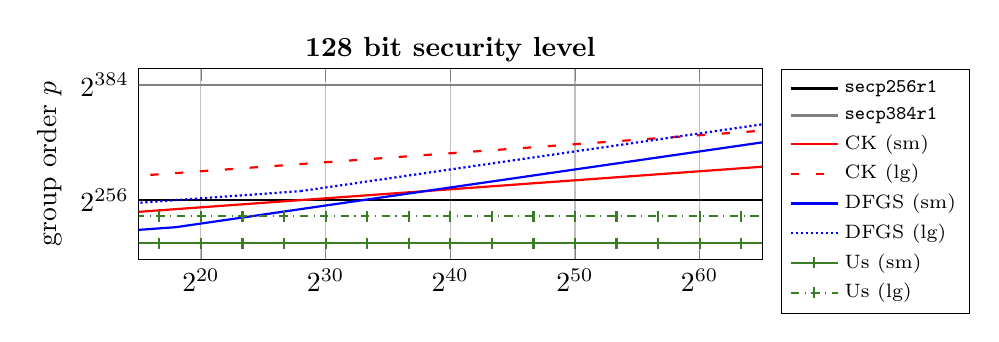
\begin{tikzpicture}
		\begin{loglogaxis}[
			title = {\textbf{128 bit security level}},
			title style  = {at={(0.5,0.9)}}, % move title a little closer to the canvas
			width=9.5cm,height=4cm,
% 			xlabel={number of sessions $\#S$}, %% only show below 2nd graph
			xmin=2^15,xmax=2^65,
			xtickten={20,30,40,50,60},
			log basis x={2},
			ylabel={group order~$p$},
			log basis y={2},
			ytickten={256,384,521},
			xmajorgrids=true,
			%
			%% legend: only printed with first plot
			legend pos=outer north east,
% 			legend style={at={(1,-0.25)},anchor=north},
% 			legend columns=-1,
			legend style={font=\scriptsize},
			legend cell align=left,
		]
		
		% NIST curves p256, p384, p521
		\addplot [black,thick,domain=1:2^80] {2^256};
		\addlegendentry{\texttt{secp256r1}}
		\addplot [gray,thick,domain=1:2^80] {2^384};
		\addlegendentry{\texttt{secp384r1}}
% 		\addplot [gray,thick,domain=1:2^80] {2^521};
% 		\addlegendentry{\texttt{secp521r1}}
		
		%% smaller-resource (sm) parameters
		% t = 2^60, #RO = 2^50, #U = 2^20 ==> adv = 2^-68
		% kl = ol = nl = 256
		% 
		%% larger-resource (lg) parameters
		% t = 2^80, #RO = 2^70, #U = 2^30 ==> adv = 2^-48
		% kl = ol = nl = 256
		% 
		
		%%%%%% CK
		\addplot[red,thick,domain=1:2^80] {(2^20*(2^20+1)*x*2^120*2^68}; % CK sm, sig dominates
		\addlegendentry{CK (sm)}
		\addplot[red,loosely dashed,thick,domain=1:2^80] {2^30*(2^30+1)*x*2^160*2^48)}; % CK lg, sig dominates
		\addlegendentry{CK (lg)}
		
		%%%%%% DFGS
		%%% sm: sig dominates for qs <= 2^18; prfodh dominates for 2^18 <= qs <= 2^68; unsatisfiable for qs >= 2^68
		\addplot[blue,thick,domain=1:2^18,forget plot]{2^20*x*2^120*2^68}; % "forget plot" to not make it appear twice in legend
		\addplot[blue,thick,domain=2^18:2^68] {x^2*4*(2^60)^2*2^68};
		\addlegendentry{DFGS (sm)}
		
		%%% lg: sig dominates for qs <= 2^28; prfodh dominates for 2^28 <= qs <= 2^68; unsatisfiable for qs >= 2^68
		\addplot[blue,densely dotted,thick,domain=1:2^28,forget plot]{2^30*x*2^160*2^48}; % "forget plot" to not make it appear twice in legend
		\addplot[blue,densely dotted,thick,domain=2^28:2^68]{x^2*4*(2^80)^2*2^48};
		\addlegendentry{DFGS (lg)}
		
		%%%%%% Us
		\addplot[OliveGreen,mark=|,thick,domain=1:2^80] {2^20*2^120*2^68}; % Us sm, sig dominates
		\addlegendentry{Us (sm)}
		\addplot[OliveGreen,dashdotted,mark=|,mark options={solid},thick,,domain=1:2^80] {2^30*2^160*2^48}; % Us lg, sig dominates
		\addlegendentry{Us (lg)}
		
		\end{loglogaxis}
		\end{tikzpicture}
	\end{minipage}
	\begin{minipage}{\textwidth}
		
		%
		% 192 bit security
		%
		
		\hspace{2cm}
		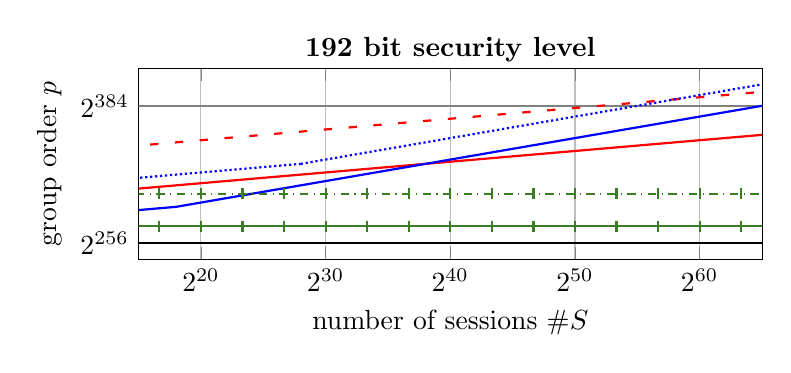
\begin{tikzpicture}
		\begin{loglogaxis}[
			title = {\textbf{192 bit security level}},
			title style  = {at={(0.5,0.9)}}, % move title a little closer to the canvas
			width=9.5cm,height=4cm,
			xlabel={number of sessions $\#S$},
			xmin=2^15,xmax=2^65,
			xtickten={20,30,40,50,60},
			log basis x={2},
			ylabel={group order~$p$},
			log basis y={2},
			ytickten={256,384,521},
			xmajorgrids=true,
			%legend pos=outer north east,
		]
		% NIST curves p256, p384, p521
		\addplot [black,thick,domain=1:2^80] {2^256};
% 		\addlegendentry{\texttt{secp256r1}}
		\addplot [gray,thick,domain=1:2^80] {2^384};
% 		\addlegendentry{\texttt{secp384r1}}
% 		\addplot [gray,thick,domain=1:2^80] {2^521};
% 		\addlegendentry{\texttt{secp521r1}}
	
		%% smaller-resource (sm) parameters
		% t = 2^60, #RO = 2^50, #U = 2^20 ==> adv = 2^-132
		% kl = ol = 384, nl = 256
		% 
		%% larger-resource (lg) parameters
		% t = 2^80, #RO = 2^70, #U = 2^30 ==> adv = 2^-112
		% kl = ol = 384, nl = 256
		% 
		
		%%%%%% CK
		\addplot[red,thick,domain=1:2^80] {(2^20*(2^20+1)*x*2^120*2^132}; % CK sm, sig dominates
		\addplot[red,loosely dashed,thick,domain=1:2^80] {2^30*(2^30+1)*x*2^160*2^112)}; % CK lg, sig dominates
		
		%%%%%% DFGS
		%%% sm: sig dominates for qs <= 2^18; prfodh dominates for 2^18 <= qs
		\addplot[blue,thick,domain=1:2^18,forget plot]{2^20*x*2^120*2^132}; % "forget plot" to not make it appear twice in legend
		\addplot[blue,thick,domain=2^18:2^80] {x^2*4*(2^60)^2*2^132};

		%%% lg: sig dominates for qs <= 2^28; prfodh dominates for 2^28 <= qs
		\addplot[blue,densely dotted,thick,domain=1:2^28,forget plot]{2^30*x*2^160*2^112}; % "forget plot" to not make it appear twice in legend
		\addplot[blue,densely dotted,thick,domain=2^28:2^80]{x^2*4*(2^80)^2*2^112};
		
		%%%%%% Us
		\addplot[OliveGreen,mark=|,thick,domain=1:2^80] {2^20*2^120*2^132}; % Ours sm, sig dominates
		\addplot[OliveGreen,dashdotted,mark=|,mark options={solid},thick,,domain=1:2^80] {2^30*2^160*2^112}; % Ours lg, sig dominates		
		\end{loglogaxis}
		\end{tikzpicture}
	\end{minipage}
	\caption[%
		Elliptic curve group order required to achieve 128-bit and 192-bit AKE security for \SIGMA and TLS~1.3
		based on the CK SIGMA, DFGS TLS~1.3, and our bounds.
	]{%
		Elliptic curve group order (y axis) required to achieve 128-bit (top) and 192-bit (bottom) AKE security for \SIGMA and TLS~1.3
		based on the CK~\protect{\cite{C:CanKra02}} SIGMA, DFGS~\protect{\cite{JC:DFGS21}} TLS~1.3, and our bounds (ours giving the same result for \SIGMA and TLS~1.3),
		for a varying number of sessions~$\# S$ (x axis).
		Both axes are in log-scale.\\
		%
		For each security and bound, we plot a smaller-resource ``(sm)'' setting with runtime $t = 2^{60}$, number of users $\# U = 2^{20}$, and number of random oracle queries $\# RO = 2^{50}$ and a larger-resource ``(lg)'' setting with $t = 2^{80}$, $\# U = 2^{30}$, and $\# RO = 2^{70}$.
		We let symmetric key/output lengths be $256$~bits for $128$-bit security and $384$-bits for $192$-bit security; nonce length is $256$~bits. 
		The group orders of NIST elliptic curves \texttt{secp256r1} ($p \approx 2^{256}$) and \texttt{secp384r1} ($p \approx 2^{384}$) are shown as horizontal lines for context.
	}
\end{figure}

\iffull
\paragraph{Numerical advantage bounds for CK, DFGS, and ours}
\else
\subsubsection*{Numerical advantage bounds\lncsdot}
\fi

We report the numerical advantage bounds for \SIGMA and TLS~1.3 based on prior (CK~\cite{C:CanKra02}, DFGS~\cite{JC:DFGS21}) and our bounds when ranging over the full parameter space detailed above in Table~\ref{tbl:bounds-full:symmetric-256-384}.
%in Tables~\ref{tbl:bounds-full:symmetric-variable} and~\ref{tbl:bounds-full:symmetric-256} (on pages~\pageref{tbl:bounds-full:symmetric-variable} and~\pageref{tbl:bounds-full:symmetric-256} in the appendix).
Table~\ref{tbl:bounds-overview} summarizes the key data points for 128-bit and 192-bit security levels.

Throughout Table~\ref{tbl:bounds-full:symmetric-256-384}, we assume that an adversary with running time $t$ makes no more than $t \cdot 2^{-10}$ queries to its random oracles.
We target the bit-security of whatever curve we use; this means that for $b$ bits of security we want an advantage of $t/2^b$.
If a bound does not achieve this goal, we color it red.
We consider runtimes between $2^{40}$ and $2^{80}$,
a total number of users between  to vary between $2^{20}$ and $2^{30}$,
and a total number of sessions between $2^{35}$ and $2^{55}$ (see above for the discussion of these parameter choices).
We evaluate these parameters in relation to all of the elliptic curve groups standardized for use with TLS~1.3.
We idealize symmetric primitives, assuming the use of $256$-bit keys in conjunction with $128$-bit security curves and $384$-bit keys in conjunction with higher-security curves,
this corresponds to the available SHA-256 and SHA-384 functions in TLS~1.3.
The nonce length is fixed to $256$~bits (as in TLS~1.3).

Our bounds do better than the CK~\cite{C:CanKra02} and DFGS~\cite{JC:DFGS21} bounds across all considered parameters and always meet the security targets,
which these prior bounds fail to meet for \texttt{secp256r1} and~\texttt{x25519} for almost all parameters,
but notably also for the $192$-bit security level of curve \texttt{secp384r1} for large-scale parameters.
We improve over prior bounds by at least~$20$ and up to~$85$ bits of security for \SIGMA,
and by at least~$35$ and up to~$92$ bits of security for TLS~1.3.

In comparison, the TLS~1.3 bounds from the concurrent work by Diemert and Jager~\cite{JC:DieJag20} yield bit security levels similar to ours for TLS~1.3:
While some sub-terms in their bound are slightly worse (esp.\ for strong DH), the dominating sub-terms are the same.



\iffull
\paragraph{Group size requirements based on CK, DFGS, and our bound}
\else
\subsubsection*{Group size requirements}
\fi

Finally, let us take a slightly different perspective on what the prior and our bounds tell us:
Figure~\ref{fig:required-groupsize} illustrates the group size required to achieve 128-bit resp.\ 192-bit AKE security for \SIGMA and TLS~1.3 based on the different bounds,
dependent on a varying number of sessions~$\#S$.
The CK \SIGMA and our \SIGMA and TLS~1.3 bounds are dominated by the signature scheme advantage (with a $\#S \cdot (\#U)^2$ loss for CK and a $\#U$ loss for our bound);
the DFGS TLS~1.3 bound instead is mostly dominated by the $(\#S)^2$--loss reduction to strong DH.
The CK and DFGS bounds require the use of larger, less efficient curves to achieve 128-bit security even for $2^{35}$ sessions.
For large-scale attackers, they similarly require a larger curve than \texttt{secp384r1} above about $2^{55}$ sessions.
We highlight that, in contrast, with our bounds a curve with 128-bit, resp. 192-bit, security is sufficient to guarantee the same security level for \SIGMA and TLS~1.3, for both small- and large-scale adversaries and for very conservative bounds on the number of sessions.




% \fg{Some numbers:}
%\begin{itemize}
%	\item \cite{C:FucKilLos18} gives an algebraic group model reduction from StrongDH to Dlog with loss $4 \qstDH$ ($\qstDH$ = number of stDH queries).
%	\item \cite{ECRYPTII-report} ``The best known algorithm for gap-CDH is to actually solve the CDH.'' -- Best-known for CDH/DDH is solving discrete log.
%	\item \cite{EC:Shoup97,IMA:Maurer05} In the generic group model, Dlog, CDH, and DDH are $(\varepsilon = t^2/p, t)$ hard (for group order~$p$, modulo small constant factors). 
%	\item In the generic group model, strongDH is also $(\varepsilon =t^2/p,t)$ hard.\hd{Try to see if we can establish a similar bound for strongDH.}
%	
%	\item \fg{We could consider two variants. (1) Conservatively assuming StrongDH algebraic reduction gap actually materializes, so considering the factor~$q$. (2) Going off the best known algorithm, in which case StrongDH and DDH are equally hard.}
%	
%	\item \fg{Stupid question: why isn't the $\tfrac{\qSend^2}{2q}$ bound problematic? (Maybe it's getting late...)}
%\end{itemize}
%


%\subsection*{fg collecting Internet-scale figures}
%
%\begin{itemize}
%	\item Let's Encrypt \url{https://letsencrypt.org/stats/} reports 130 million $\approx 2^{27}$ active certs as of May 13, 2020.
%	\item BuiltWith \url{https://trends.builtwith.com/ssl/traffic/Entire-Internet} reports 160 million $\approx 2^{27}$ certificates on the Internet.
%	\item \url{https://www.internetlivestats.com/} reports 4.5 billion ($2^{32}$) Internet users, 7 billion Google searches \emph{per day} ($2^{33}$)
%	\item Qualys SSL Pulse \url{https://www.ssllabs.com/ssl-pulse/} reports 29.7\% of the 150K top Alexa sites support TLS~1.3.
%	\item ITU \url{https://www.itu.int/en/ITU-D/Statistics/Pages/stat/default.aspx} estimates 4.1 billion Internet users in 2019.
%\end{itemize}


% \subsection*{fg: Parameters and Building Blocks}
% 
% Elliptic curve groups in TLS~1.3
% 
% % \begin{table}
% % 	\centering
% {
% % 	\renewcommand{\tabcolsep}{0.25cm}
% 	\begin{tabular}{@{}llll@{}}
% 		\toprule
% 		Group			& bit-security	& order $p$		& DH time \\
% 		\midrule
% 		\texttt{secp256r1}	& 128		& $\approx 2^{256}$	& \\
% 		\texttt{secp384r1}	& 192		& $\approx 2^{384}$	& 2x p256 \footnotemark \\
% 		\texttt{secp521r1}	& 256		& $\approx 2^{518}$	& 4x p521 \addtocounter{footnote}{-1}\footnotemark \\
% 		\texttt{x25519}		& 128		& $\approx 2^{252}$	& \\
% 		\texttt{x448}		& 224		& $\approx 2^{446}$	& 5x x25519 \cite{SAC:OLHFR17} \\
% 		\bottomrule
% 	\end{tabular}
% }
% % 	\caption{Elliptic curve groups in TLS~1.3}
% % \end{table}
% 	\footnotetext{\url{https://csrc.nist.gov/csrc/media/events/lightweight-cryptography-workshop-2015/documents/presentations/session7-vincent.pdf}}
% 
% \bigskip
% \noindent
% Signature algorithms in TLS~1.3
% 
% % \begin{table}
% % 	\centering
% {
% 	\renewcommand{\tabcolsep}{0.25cm}
% 	\begin{tabular}{@{}lll@{}}
% 		\toprule
% 		Algorithm				& bit-security	& \\
% 		\midrule
% 		\texttt{ecdsa\_secp256r1\_sha256}	& 128		& \\
% 		\texttt{ecdsa\_secp384r1\_sha384}	& 192		& \\
% 		\texttt{ecdsa\_secp521r1\_sha512}	& 256		& \\
% 		\texttt{ed25519}			& 128 \cite{rfc8032}		& \\
% 		\texttt{ed448}				& 224 \cite{rfc8032}		& \\
% 		\texttt{rsa\_pss\_pss\_sha256}		& 		& \\
% 		\texttt{rsa\_pss\_pss\_sha384}		& 		& \\
% 		\texttt{rsa\_pss\_pss\_sha512}		& 		& \\
% 		\bottomrule
% 	\end{tabular}
% }
% % 	\caption{Signature schemes in TLS~1.3}
% % \end{table}
